\begin{figure}[h]
    \centering
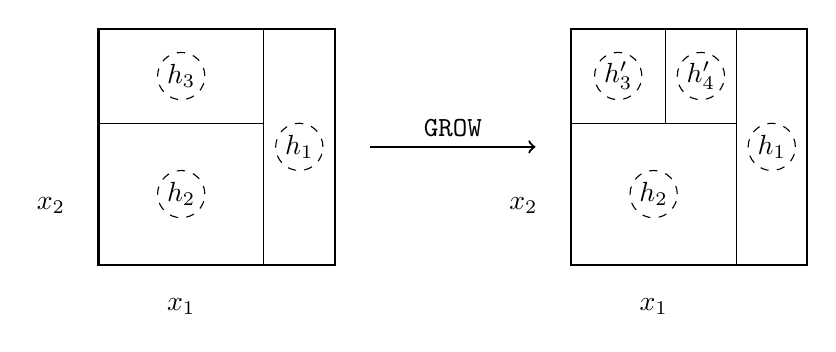
\begin{tikzpicture}[scale=3] % Increase scale for a larger square
    % Left square
    % Define the unit square
    \draw[thick] (0, 0) rectangle (1, 1);
    
    % Vertical line at x1 = 0.7
    \draw[thin] (0.7, 0) -- (0.7, 1) ;
    
    % Horizontal line at x2 = 0.6
    \draw[thin] (0, 0.6) -- (0.7, 0.6);
    
    % Labels for axes
    \node[below] at (0.35, -0.1) {$x_1$};
    \node[left] at (-0.1, 0.25) {$x_2$};

    % Splitting variables of the partition
    % \node[right] at (1.05, 0.6)  {\small{$x_2 = 0.6$}};
    % \node[above] at (0.7, 1.05)  {\small{$x_1 = 0.7$}};
    
    % Step heights
    \node at (0.85, 0.5) {$h_1$};
    \node at (0.35, 0.3) {$h_2$};
    \node at (0.35, 0.8) {$h_3$};

    % Circles around step heights
    \draw[dashed] (0.85, 0.5) circle [radius=0.10];
    \draw[dashed] (0.35, 0.3) circle [radius=0.10];
    \draw[dashed] (0.35, 0.8) circle [radius=0.10];
    
    % Right squares
    % First square (top)
    \begin{scope}[shift={(2.0, 0.0)}]
        \draw[thick] (0, 0.00) rectangle (1, 1);
    
        \draw[thin] (0.7, 0) -- (0.7, 1);
        \draw[thin] (0, 0.6) -- (0.7, 0.6);
        \draw[thin] (0.4, 0.6) -- (0.4, 1.0);
        
        % Step heights
        \node at (0.85, 0.5) {$h_1$};
        \node at (0.35, 0.3) {$h_2$};
        \node at (0.55, 0.8) {$h_4'$};
        \node at (0.2, 0.8) {$h_3'$};
    
        % Circles around step heights
        \draw[dashed] (0.85, 0.5) circle [radius=0.10];
        \draw[dashed] (0.35, 0.3) circle [radius=0.10];
        \draw[dashed] (0.55, 0.8) circle [radius=0.10];
        \draw[dashed] (0.2, 0.8) circle [radius=0.10];

        \node[below] at (0.35, -0.1) {$x_1$};
        \node[left] at (-0.1, 0.25) {$x_2$};
    \end{scope}

    
    % Arrows from the left square to each of the right squares
    \draw[->, thick] (1.15, 0.5) -- (1.85, 0.5) node[midway, sloped, above] {\texttt{GROW}}; 
\end{tikzpicture}
\caption{Illustration of a \texttt{GROW} move: the left panel shows the original covariate partition, and the right panel shows the updated partition with one additional split and two new step heights.}
\label{fig:partition_grow}
\end{figure}




